\Chapter{}
\chapter{METODOLOGÍA}
    \section{Área de estudio}
        La investigación se enfocó en imágenes Landsat MSS y TM de diversas regiones a nivel mundial. La Antártida se excluye por su homogeneidad espectral, dominada por extensas áreas de hielo y nieve, lo que dificulta la diferenciación de coberturas y complica la armonización satelital \autocite{kokhanovsky2019retrieval}. De manera similar, las regiones oceánicas se descartan debido a su uniformidad espectral, lo que limita la variabilidad en la reflectancia \autocite{estrella2021spectral}. Por lo tanto, el estudio se centra en áreas continentales no homogéneas en términos de reflectancia.
        \begin{figure}[H] 
            \caption{\doublespacing \\ \textit{Mapa del área de estudio.}} 
            \centering
            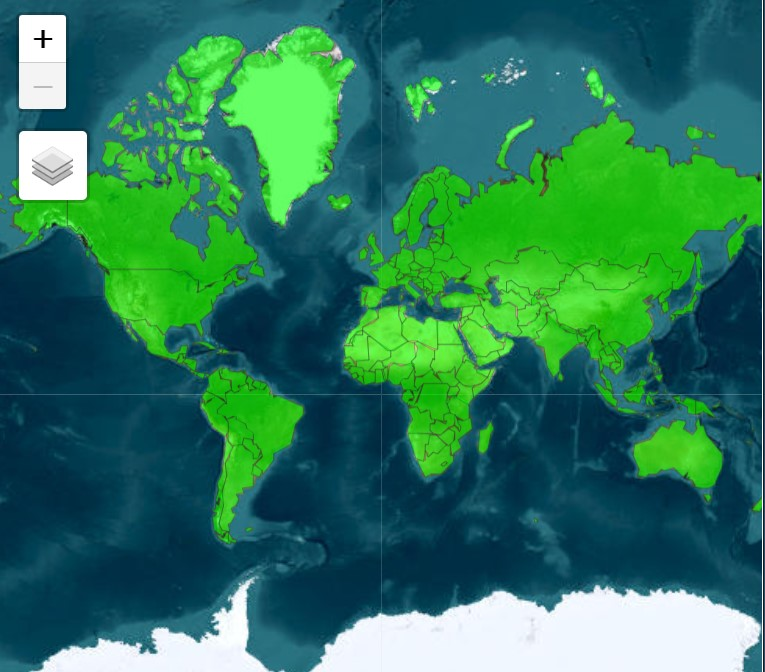
\includegraphics[width=0.6\linewidth]{E_IMAGENES/area_estudio.jpg}
            \begin{justify}
                \textit{Nota.} Se muestra un mapa satelital global, resaltando las zonas terrestres verdes, omitiendo océanos uniformes y la helada Antártida.
            \end{justify}                    
            \label{area_estudio}
        \end{figure}
    \section{Diseño de investigación}
        \subsection{Tipo de investigación}
            Aplicada, ya que tiene como objetivo principal utilizar técnicas avanzadas de inteligencia artificial para mejorar la armonización de las imágenes Landsat MSS. La finalidad es proporcionar herramientas más eficientes y precisas para el monitoreo global, beneficiando a investigadores, entidades gubernamentales y organizaciones relacionadas con el estudio de la superficie terrestre.
        \subsection{Nivel de investigación}
            Descriptiva y exploratoria. Es descriptiva porque se analizarán las características y ventajas de las técnicas de aprendizaje profundo en la armonización de imágenes MSS. Es exploratoria, ya que se busca comprender y evaluar cómo estas técnicas pueden mejorar la calidad y precisión de estas imágenes, un área con desafíos y oportunidades para la innovación.
	\subsection{Enfoque}
            Cuantitativo. Se utilizarán herramientas y técnicas estadísticas para evaluar la eficacia de las técnicas de aprendizaje profundo en la armonización de las imágenes. Esto implica comparar imágenes antes y después de la armonización, evaluando la calidad de las imágenes resultantes y cotejándolas con métodos tradicionales. Los resultados se expresarán numéricamente, utilizando indicadores como porcentajes de mejora, errores cuadráticos medios, entre otros relevantes.

    \section{Población y muestra}
    
        \subsection{Población}
            La población objeto de este estudio consiste en la totalidad de las imágenes obtenidas por el sensor MSS del satélite Landsat que cubren las regiones continentales globales, excluyendo la Antártida y las regiones oceánicas, durante el período de tiempo comprendido entre 1982 y 1999. Estas imágenes están disponibles a través de las bases de datos de Landsat, las cuales proporcionan un registro histórico completo y accesible para la extracción de los datos necesarios para el presente estudio.

        \subsection{Muestra}
            El diseño de muestreo adoptado es de tipo probabilístico. Se seleccionarán unidades de muestreo de manera aleatoria, lo cual es esencial para garantizar la independencia estadística y la representatividad dentro del universo de las imágenes MSS de Landsat. De acuerdo con los principios establecidos por \textcite{hernandez2014recoleccion}, se ha determinado un tamaño de muestra representativo del conjunto total de la población.

            Para la implementación de la superresolución MSS a TM mediante el modelo ESRGAN, se implementaron técnicas de clasificación supervisada, que requieren un conjunto de datos dividido en muestras de entrenamiento y validación.
            Siguiendo las recomendaciones de \textcite{belgiu2016random}, las muestras de entrenamiento deben ser: 1) estadísticamente independientes de las muestras de validación, 2) equilibradas en términos de distribución de clases, 3) representativas de las variabilidades espectrales objetivo, y 4) suficientemente amplias para cubrir la complejidad de los datos. Con base en estos criterios, para este estudio se destinará el 70\% de las imágenes seleccionadas aleatoriamente para el entrenamiento del modelo y el 30\% restante para la validación del mismo \autocite{nami2018spatial}. La asignación de las imágenes a cada uno de estos conjuntos se realizará mediante un algoritmo de selección aleatoria que asegure la aleatoriedad de la división \autocite{gigovic2019testing}.

            Además, se incorporó la especificación ML-STAC para estructurar y describir los datos de EO de manera óptima para el entrenamiento de modelos de ML. Se utilizó este estándar para convertir los datos en el formato safetensor y cargarlos en la plataforma Hugging Face, permitiendo un acceso eficiente y reproducible a los datos curados. Este enfoque garantiza una mayor coherencia, transparencia y facilita la verificación independiente de los resultados del estudio.
        
    \section{Procedimiento, técnicas e instrumentos de recolección de información}

       \subsection{Obtención de datos de entrada}
            \subsubsection{Selección por localización}
                Para garantizar la eficacia y precisión de la investigación, se llevó a cabo una meticulosa selección de imágenes para el estudio. A continuación, se detalla el procedimiento de selección:
                
                \begin{enumerate}
                    \item Como punto de partida, se generaron puntos de manera aleatoria alrededor del mundo, resultando en un total inicial de 20 000 puntos. Estos puntos sirvieron como centroides para definir buffers cuadrados con dimensiones de 30 720 metros por lado.
                    
                    \begin{figure}[H] 
                        \caption{\doublespacing \\ \textit{Generación de 20 000 puntos aleatorios a nivel mundial.}} 
                        \centering
                        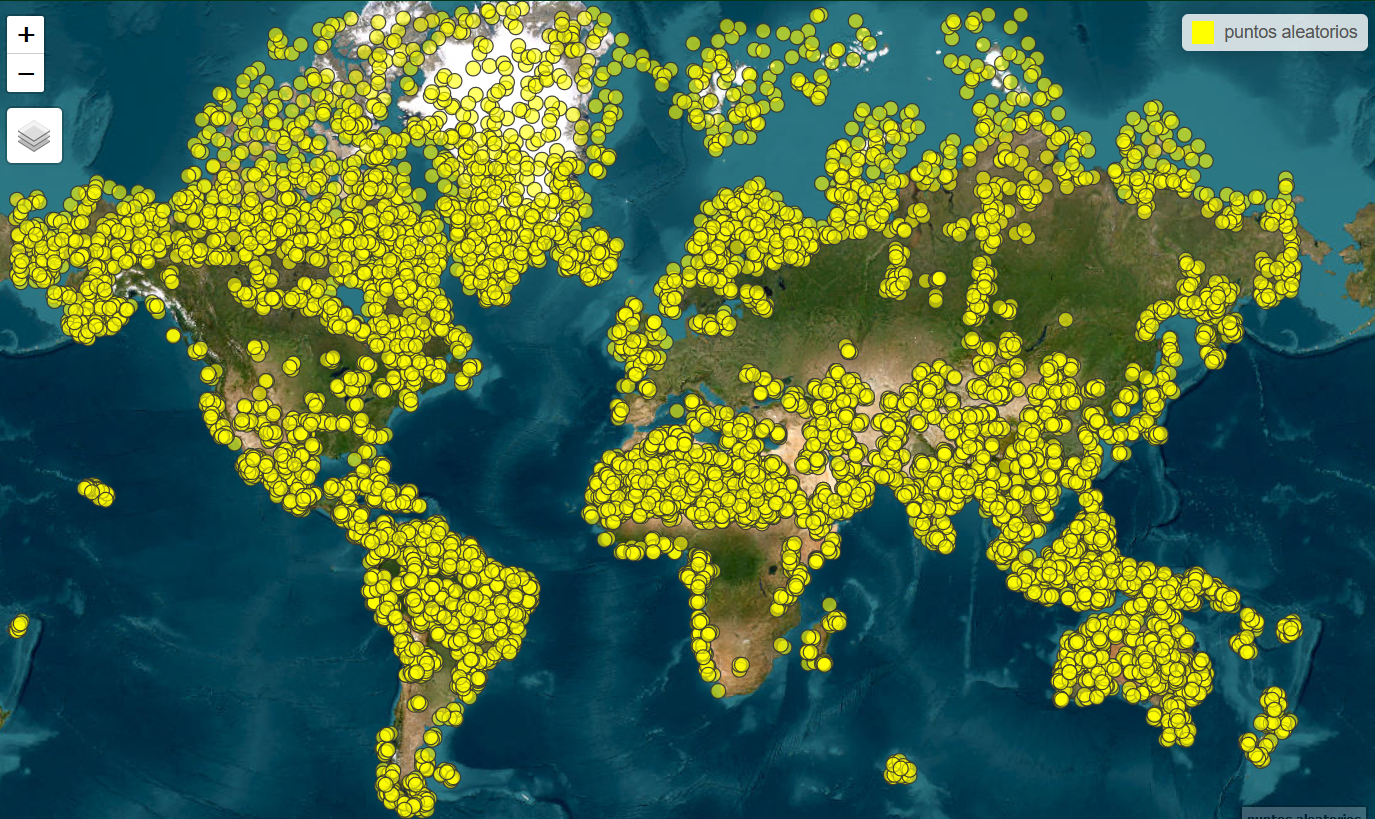
\includegraphics[width=0.7\linewidth]{2_CAPITULO0/IMG/1000points.png}
                        \begin{justify}
                            \textit{Nota.} Los puntos no excedieron los límites del WRS-2 (desde Landsat 4 hasta Landsat 9), que corresponden a las áreas o segmentos de captura de todas las imágenes Landsat, incluyendo los sensores más recientes.
                        \end{justify}                    
                        \label{1000points}
                    \end{figure}

        
                    \item Con los puntos geográficos establecidos, se procedió a seleccionar imágenes específicas. Se optó por imágenes MSS pertenecientes exclusivamente a las misiones Landsat 4 y 5, ya que coinciden con las imágenes obtenidas por el sensor TM de las mismas misiones durante el período de 1982 a 1999.
                
                    \item Una condición crucial en esta fase fue asegurar que el área definida por cada buffer estuviera íntegramente contenida dentro de al menos una imagen MSS y una imagen TM. Este criterio busca prevenir truncamientos o limitaciones en la amplitud de las imágenes.
                    
                    \item Se excluyeron ciertas áreas geográficas del proceso: específicamente, regiones de la Antártida y zonas mayormente oceánicas, para asegurar la relevancia y calidad del conjunto de datos final.
                    
                    \item Tras aplicar todos los criterios anteriores, de los 20 000 puntos iniciales, solo 19 546 satisfacían todas las condiciones y, por lo tanto, fueron retenidos para el estudio.
                \end{enumerate}
            \subsubsection{Selección por tiempo y calidad}
                Tras el filtro geográfico inicial, se procedió a una selección más detallada basada en criterios temporales y de calidad. A continuación se describe el procedimiento adoptado:
                
                \begin{enumerate}
                    \item De los 20 000 puntos iniciales, solo 19 546 cumplían con los criterios de localización. Para estos puntos seleccionados, se llevó a cabo una comparación temporal entre las imágenes de ambos sensores.
                
                    \item La condición impuesta fue que las imágenes de ambos sensores debían tener un diferencial temporal no superior a 10 minutos. Es decir, por cada punto, se retuvieron solo aquellos pares que hubieran sido capturadas en un intervalo de tiempo menor o igual a 10 minutos entre ellas.
                    
                    \item Es importante mencionar que este filtro temporal se aplicó considerando imágenes de los niveles Tier 1 y Tier 2 para ambos sensores. Debido a este riguroso criterio, no todos los puntos conservaron la misma cantidad de imágenes, y algunos incluso quedaron sin imágenes que cumplieran con este requisito.
                    
                    \item Posterior al filtro temporal, se implementó un filtro de calidad basado en la nubosidad. Se utilizó la banda de calidad (QA), específicamente de las imágenes del sensor TM, para evaluar la presencia de nubes o sombras. El criterio adoptado fue que las imágenes retenidas no debieran tener una cobertura de nubes o sombras que superara el 15\% del área del buffer generado por el punto dentro de la extensión de la imagen.
                    
                    \item Al concluir estos filtros, se obtuvo un conjunto final de imágenes (15 878 pares) filtradas que satisfacen tanto los criterios de diferencial temporal como los de calidad en relación con la nubosidad.
                \end{enumerate}
                
                Este enfoque garantizó un conjunto de datos con alta precisión temporal y calidad visual, minimizando las distorsiones o interferencias potenciales debido a la nubosidad.

  
        \subsection{Corrección geométrica de las Imágenes MSS}
            El propósito de este proceso es asegurar una alineación precisa entre las imágenes MSS y TM. A continuación, se detallan las etapas de la corrección geométrica:
            
            \subsubsection{Lectura y Preprocesamiento de Imágenes}
                Se cargan las imágenes, y son normalizadas para tener valores reales de reflectancia. Se seleccionan únicamente las bandas que coinciden entre las imágenes, garantizando su comparabilidad.
            
            \subsubsection{Extracción y Coincidencia de Características}
                Con la ayuda de modelos de aprendizaje profundo como LightGlue, se identifican puntos clave en ambas imágenes. Estos puntos son luego emparejados para determinar la desalineación entre las imágenes MSS y TM.
                
                \begin{figure}[H] 
                    \caption{\doublespacing \\ \textit{LightGlue: Emparejamiento de Características en Imágenes con Mecanismo Adaptativo.}} 
                    \centering
                    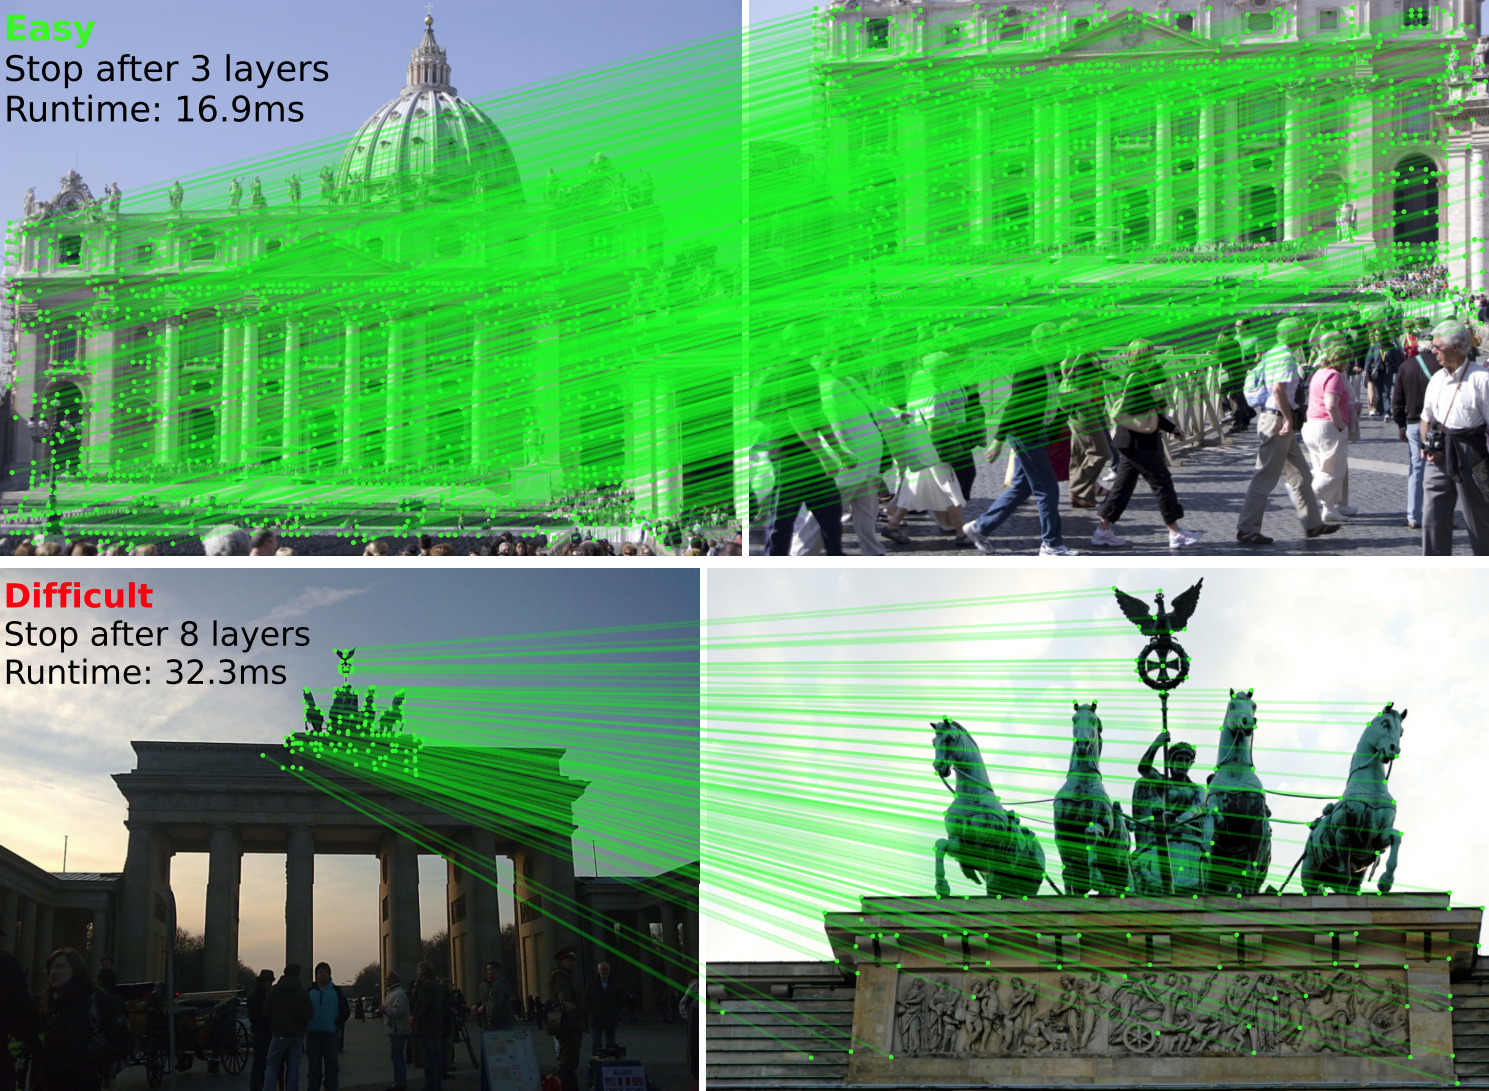
\includegraphics[width=0.7\linewidth]{2_CAPITULO0/IMG/cvg.png}
                    \begin{justify}
                        \textit{Nota.} La interfaz de 'LightGlue' exhibe dos ejemplos: uno 'fácil' con características emparejadas del Vaticano en 16.9ms y tres capas de procesamiento, y otro "difícil" de un monumento con estatuas, procesado en 32.3ms y ocho capas. Obtenido de \textcite{LightGlue2023}.
                    \end{justify}                    
                    \label{cvg}
                \end{figure}
                
               
            \subsubsection{Determinación del Desplazamiento Espacial}
                Usando los puntos clave coincidentes, se estima el desplazamiento espacial entre las imágenes. Este desplazamiento señala cuánto y cómo se desalinean las imágenes en términos de píxeles.

                \begin{figure}[H] 
                    \caption{\doublespacing \\ \textit{Emparejamiento Adaptativo de Características con LightGlue: De Alta Resolución (HR) a Baja Resolución (LR).}} 
                    \centering
                    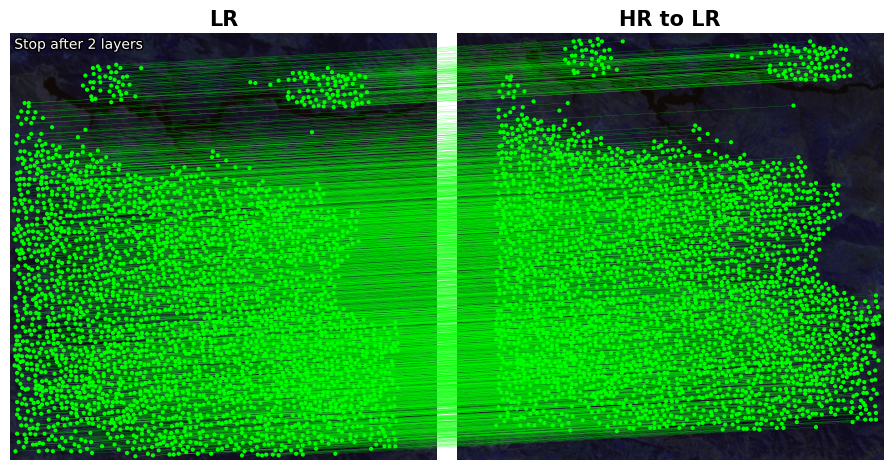
\includegraphics[width=0.8\linewidth]{2_CAPITULO0/IMG/hr_to_lr.png}
                    \begin{justify}
                        \textit{Nota.} Se observan superposiciones verdes de características detectadas, deteniéndose en ambas tras dos capas, evidenciando la eficacia de "LightGlue".
                    \end{justify}                    
                    \label{hr_to_lr}
                \end{figure}
                
            \subsubsection{Refinamiento Subpíxel y Convolución en 2D}
                Para refinar la corrección, se recurre a la transformada de Fourier. Esta técnica, mediante la función de correlación cruzada en el dominio de frecuencia, equivale a una convolución en 2D en el dominio espacial. La convolución en 2D es una operación que toma dos imágenes de entrada y produce una tercera imagen como salida, siendo una técnica fundamental en procesamiento de imágenes para filtrar y enfocar. Aquí, ayuda a identificar desplazamientos subpíxeles basados en el contenido de frecuencia de las imágenes.
                
                \begin{equation}
                    X(f) = \int_{-\infty}^{\infty} x(t) \cdot e^{-j2\pi ft} dt
                \end{equation}
            
                Donde \(X(f)\) es la transformada de Fourier de la señal \(x(t)\).
                
                
                Con base en el desplazamiento determinado y su refinamiento subpíxel, las imágenes MSS son alineadas geométricamente con las TM.
                
                Las imágenes MSS corregidas se presentan junto con las TM para confirmar visualmente la alineación. A través del proceso de corrección, se observa una mejora notable en la alineación, evidenciada por la reducción del desajuste visual entre las imágenes. Esta mejora se logra mediante correcciones tanto a nivel de píxel como subpíxel, lo que resulta en una superposición más precisa entre las imágenes MSS y TM.
                
                \begin{figure}[H] 
                    \caption{\doublespacing \\ \textit{Comparativa de Alineación: Imágenes MSS, TM y MSS Corregida.}} 
                    \centering
                    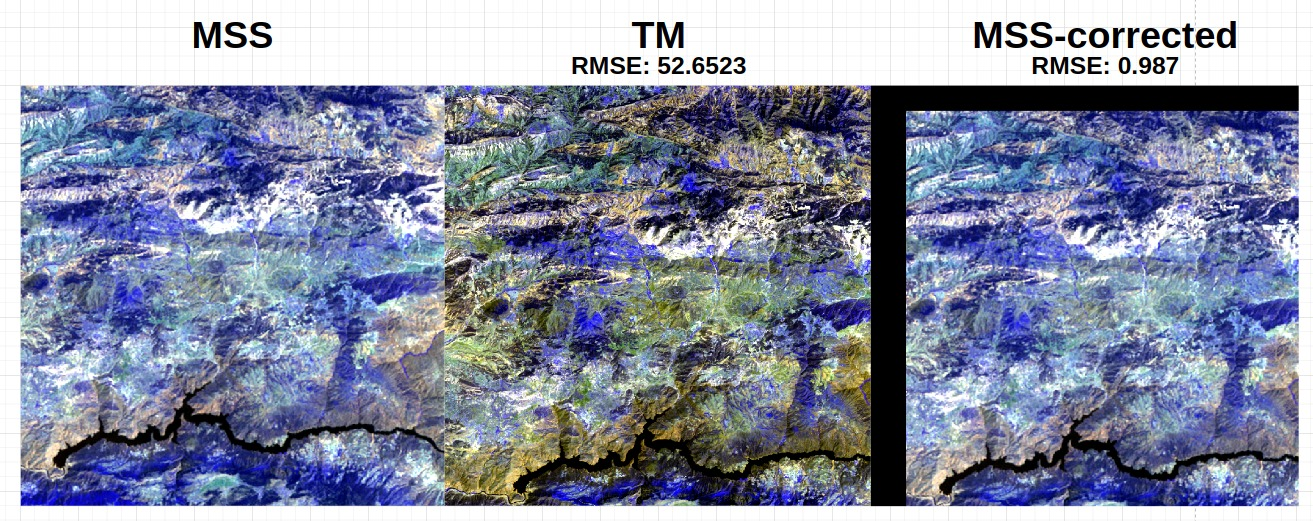
\includegraphics[width=0.8\linewidth]{2_CAPITULO0/IMG/tm_mss_rmse.png}
                    \begin{justify}
                        \textit{Nota.} El contraste entre la imagen MSS original y la corregida resalta con una reducción significativa del error RMSE de 52.6523 a 0.987, evidenciando la eficacia de las correcciones a nivel de píxel y subpíxel para lograr una alineación casi perfecta.
                    \end{justify}                    
                    \label{tm_mss_rmse}
                \end{figure}
                
            \subsubsection{Filtro final de los pares de imágenes}
                En complemento a las técnicas previamente descritas, se incorpora un criterio adicional para la exclusión de correspondencias erróneas entre las imágenes. Se establece un umbral de exclusión para desplazamientos que superen los 90 metros, equivalentes a 3 píxeles, con el objetivo de asegurar realismo y precisión en la alineación, descartando así anomalías significativas. Este enfoque resulta esencial debido a discrepancias previamente observadas entre las ubicaciones de las imágenes MSS y la realidad, utilizando como referencia las imágenes TM. Para optimizar el proceso, se implementa un filtro automatizado en lugar de una revisión visual individual.

                Posteriormente, se calcula el error cuadrático medio de colocación con los puntos restantes, un paso crítico para evaluar la precisión en la alineación de las imágenes MSS de baja resolución (LR) con las TM de alta resolución (HR). Se decide excluir del análisis cualquier par de imágenes cuyo error supere los 0.75 píxeles, con el fin de garantizar una alineación de alta precisión y minimizar desajustes residuales.
            
                Este rigor en la selección asegura la retención en el conjunto de datos únicamente de aquellas imágenes con una alineación casi perfecta, incrementando así la confiabilidad de los resultados. La combinación de este criterio con las correcciones a nivel de píxel y subpíxel conduce a una mejora notable en la alineación de las imágenes MSS y TM, reflejada en una reducción significativa del error RMSE.
            
                Finalmente, tras aplicar estos criterios de selección y refinamiento, se obtuvo un conjunto final de 5431 pares de imágenes. Estos pares seleccionados constituyen la base de datos con la que se entrenará el primer modelo de armonización de bandas, proporcionando una fundación sólida y precisa para el análisis y desarrollo del modelo.
        % \subsection{Aplicación de parámetros BRDF}
            %     Siguiendo el proceso de selección y filtrado de imágenes basado en criterios de diferencial temporal y calidad en relación con la nubosidad, se procedió con la aplicación de parámetros BRDF a las imágenes Landsat MSS y TM seleccionadas. Este paso fue fundamental para ajustar las imágenes a una base común de reflectancia, considerando las variaciones angulares y de iluminación inherentes a la captura de datos de satélite.
                
            %     \subsubsection{Selección y Preparación de Imágenes}
            %         Se seleccionaron imágenes pares de MSS y TM que correspondían en términos de ubicación y tiempo. La aplicación de parámetros BRDF a estas imágenes fue crucial para homogeneizar la reflectancia, permitiendo comparaciones precisas entre ellas.

            %     \subsubsection{Procesamiento con librecubo-brdf}
            %         Para la aplicación de correcciones BRDF, se utilizó el paquete librecubo-brdf, el cual implementa el método c-factor. Este método ajusta la reflectancia de las imágenes en función de su posición respecto al nadir y la iluminación solar, alineándolas con el concepto de Nadir BRDF Adjusted Reflectance (NBAR). Esta normalización es vital para una interpretación uniforme y precisa de los datos de reflectancia.

            %     \subsubsection{Homogeneización espectral}
            %         Con la aplicación de los parámetros BRDF, las imágenes pares quedaron normalizadas en términos de reflectancia. Este ajuste aseguró que las diferencias observadas en análisis posteriores reflejaran variaciones reales en las características de la superficie terrestre, y no artefactos debidos a la variabilidad en la captura de datos.


        \subsection{Generación de Dataloader Preparación Final de Datos}
            La fase de preparación y organización de datos es fundamental en el proceso de armonización de bandas entre las imágenes de baja resolución (MSS) y alta resolución (TM). Este proceso se estructura en varias etapas clave para garantizar la calidad y eficiencia del modelo de deep learning.

            \subsubsection{Conversión de formato de datos}
                Los datos originales en formato TIFF fueron transformados al formato SafeTensor, un cambio crucial para el almacenamiento y manejo eficiente de grandes volúmenes de datos. Esta conversión facilitó un acceso más rápido y una gestión más eficaz en los procesos de aprendizaje automático.

            \subsubsection{Estandarización y homogeneización}
                Se estandarizaron los datos para garantizar una estructura uniforme y coherente. La normalización de metadatos, el uso de esquemas JSON y la estructuración detallada de los datos aseguraron la integridad y la calidad de la información procesada.

            % \subsubsection{Implementación de dataLoaders en PyTorch}
            %     La creación de dataloaders específicos en PyTorch permitió la gestión óptima de los datos. La carga y procesamiento paralelo en múltiples núcleos de CPU optimizaron el rendimiento, esencial para el manejo de grandes conjuntos de datos.

            \subsubsection{Integración con Hugging Face}
                Los datos procesados y estandarizados se alojaron en la plataforma en la nube Hugging Face, proporcionando un acceso accesible y compartible. Esta integración facilitó la colaboración y el acceso a los datos para aplicaciones futuras en diversos proyectos.
            
            \subsubsection{Conversión de formato de datos}
                Con un total de 5431 pares de imágenes MSS y TM, se realiza una cuidadosa segmentación del conjunto. Esta segmentación resulta en una distribución donde aproximadamente el 81\% de los datos se asignan para entrenamiento, mientras que el 9\% se destina a la validación y otro 10\% para pruebas. Esta división equilibrada es crucial para evaluar adecuadamente la capacidad del modelo en diferentes conjuntos de datos.
            
            \subsubsection{Procesamiento y Alineación de Imágenes} 
                Cada par de imágenes pasa por un proceso de procesamiento y alineación. Se realiza una cuidadosa eliminación de píxeles de borde y se aplica un recorte aleatorio para generar muestras de 256x256 píxeles en las imágenes MSS. Para las imágenes TM, se utiliza la técnica de interpolación bilineal con antialiasing para ajustar su resolución, mejorando la calidad visual y reduciendo artefactos.
            
            \subsubsection{Normalización y Preparación de Datos} 
                Las imágenes procesadas son normalizadas para asegurar la consistencia en la escala de valores de píxeles. Esta normalización es esencial para la eficiencia del aprendizaje, asegurando que tanto las imágenes MSS como las TM contribuyan de manera equitativa al entrenamiento del modelo. 
            
            \subsubsection{Optimización y Manejo Eficiente de Datos} 
                Los dataloaders se configuran para optimizar la carga y manejo de los datos durante el entrenamiento y la validación. Se establecen parámetros específicos como el tamaño del lote y el número de hilos de procesamiento, buscando una mayor eficiencia y un uso óptimo de los recursos computacionales.
            
                \begin{figure}[H] 
                    \caption{\doublespacing \\ \textit{Flujo del Proceso de Preparación y Organización de Datos.}} 
                    \centering
                    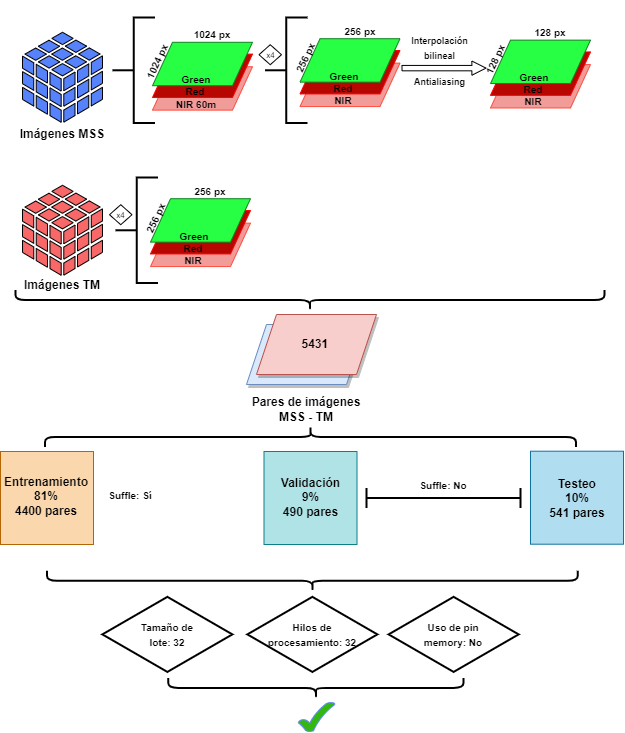
\includegraphics[width=0.8\linewidth]{2_CAPITULO4/IMG/dataloader.png}
                    \begin{justify}
                        \textit{Nota.} El gráfico detalla el flujo de datos en la preparación de imágenes satelitales MSS y TM, su segmentación en lotes y la configuración eficiente de dataloaders para el modelo.
                    \end{justify}                    
                    \label{dataloader}
                \end{figure}

                Este proceso no solo facilita el manejo eficiente de los datos, sino que también asegura que cada par de imágenes MSS y TM sea procesado y presentado al modelo de manera óptima, mejorando la precisión y efectividad del entrenamiento para la armonización de bandas.

        \subsection{Desarrollo del Modelo MSS2TM para Alineación Espacial y Espectral}
            
            \subsubsection{Configuración del Entorno de Trabajo}
                Se estableció un entorno de trabajo en Python mediante la creación de un entorno virtual utilizando herramientas como venv. Esto permitió una separación clara y la gestión de dependencias específicas del proyecto. Se instaló PyTorch, seleccionando una versión que correspondiera a la compatibilidad con CUDA del sistema utilizado, para facilitar el entrenamiento acelerado por GPU.
            
\begin{lstlisting}[language=bash]
python -m venv mss2tm-env
# Activar entorno en Windows
mss2tm-env\Scripts\activate
# Activar entorno en Unix o MacOS
source mss2tm-env/bin/activate
\end{lstlisting}
            
                Además, se implementaron herramientas de registro y monitoreo para seguir el progreso del entrenamiento y se estableció un sistema de control de versiones para el código y los datos. La automatización y orquestación del flujo de trabajo, junto con la validación del código mediante pruebas unitarias y de integración, formaron parte esencial de este proceso. Todas las dependencias se documentaron en un archivo requirements.txt para facilitar la configuración reproducible del entorno.

\begin{lstlisting}[language=bash]
# Instalación de PyTorch y bibliotecas para procesamiento de imágenes
pip install torch torchvision torchaudio
pip install numpy scipy matplotlib pandas geopandas rasterio fiona
pip install opencv-python-headless scikit-image scikit-learn

# Herramientas de desarrollo para código eficiente y limpio
pip install flake8 black isort mypy

# Bibliotecas para la manipulación y aumento de datos geoespaciales
pip install albumentations pytorch-lightning

# Control de versiones para el código y los datos
pip install git dvc

# Herramientas de registro y monitoreo
pip install tensorboard wandb

# Pruebas unitarias y de integración
pip install pytest pytest-cov

# Documentación de dependencias
pip freeze > requirements.txt
\end{lstlisting}


            \subsubsection{Diseño de la Arquitectura del Modelo}
                Para el desarrollo del modelo MSS2TM, se adoptó una arquitectura de superresolución generativa adversaria mejorada (ESRGAN). Esta elección se basó en su capacidad demostrada de producir imágenes de alta resolución con detalles realistas a partir de imágenes de baja resolución. La arquitectura se personalizó para adaptarse a las características específicas de las imágenes MSS y TM de los satélites Landsat.
                
                Para lograr una coherencia óptima entre las imágenes, es fundamental establecer una correspondencia tanto espacial como espectral entre ellas. El objetivo es convertir las imágenes MSS para que sean similares en resolución y calidad a las imágenes TM. Para ello, desarrollamos el modelo de aprendizaje profundo llamado MSS2TM. 
            
                \begin{figure}[H] 
                    \caption{\doublespacing \\ \textit{Flujo de un modelo de red neuronal ESRGAN.}} 
                    \centering
                    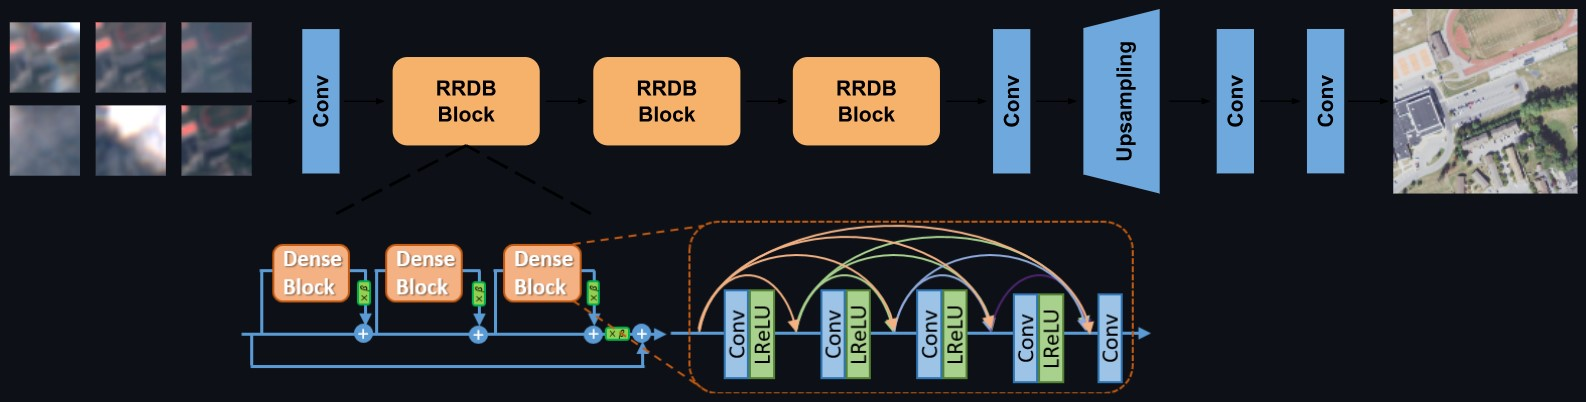
\includegraphics[width=0.9\linewidth]{E_IMAGENES/modelo_esgr.jpg}
                    \begin{justify}
                        \textit{Nota.} Se muestra un flujo de trabajo de procesamiento de imagen con bloques RRDB para mejorar resolución, con capas convolucionales, densas, activaciones LeRU y técnicas de upsampling. Obtenido de \textcite{wolters2023zooming}.
                    \end{justify}                    
                    \label{red_neuronal}
                \end{figure}

                \paragraph{Arquitectura General}
                    La red generativa de ESRGAN se compone de bloques Residual in Residual Dense Block (RRDB), que son el núcleo para aprender las representaciones residuales. Cada RRDB consta de varias capas de convolución densamente conectadas que facilitan el aprendizaje de características en múltiples niveles de abstracción. Se emplearon capas convolucionales con filtros de tamaño 3x3, siguiendo las prácticas estándar para la preservación de detalles en imágenes.
            
                \paragraph{Adaptaciones Específicas para MSS y TM}
                    La entrada de la red generativa fue modificada para aceptar las bandas espectrales específicas de las imágenes MSS de baja resolución, que luego se mapearían a las bandas correspondientes de las imágenes TM de alta resolución. Se ajustó el número de canales de entrada y salida de la red para alinearse con el número de bandas espectrales de los satélites.
            
                \paragraph{Entrenamiento y Activaciones}
                    El modelo se entrenó utilizando un conjunto de datos de pares de imágenes MSS-TM alineados espacialmente. Se utilizó la función de activación LeakyReLU, preferida por su capacidad de manejar el problema de las neuronas "muertas" mejor que la ReLU tradicional, lo que es crucial en el entrenamiento de modelos GAN. En las capas de salida, se aplicó la función de activación Tanh para mapear los valores de los píxeles a un rango normalizado, lo que ayuda en la convergencia del entrenamiento y la calidad de las imágenes generadas.
            
            \subsubsection{Configuración de las Funciones de Pérdida}
                La eficacia de un modelo de superresolución como MSS2TM depende en gran medida de las funciones de pérdida utilizadas durante el entrenamiento. Estas funciones de pérdida son cruciales para guiar el proceso de aprendizaje del modelo hacia la generación de imágenes que no solo son visualmente atractivas, sino que también son fieles a las características reales de las imágenes de alta resolución. Para el modelo MSS2TM, se adoptó un enfoque multiobjetivo en la selección y configuración de las funciones de pérdida, basándose en la naturaleza de las imágenes MSS y TM.
                    
                \paragraph{CLIPLoss}
                    La función de pérdida CLIPLoss se utilizó para evaluar la similitud perceptual entre las imágenes generadas y las de alta resolución. CLIPLoss aprovecha un modelo preentrenado de CLIP (Contrastive Language–Image Pretraining) para comparar las características visuales y contextuales de las imágenes. Esta función de pérdida es particularmente efectiva para asegurar que las imágenes superresueltas no solo coincidan en términos de píxeles, sino que también capturen con precisión los elementos y patrones semánticos presentes en las imágenes TM de alta resolución.

            \subsubsection{Creación del Dataset (Diseño y División)}

                \paragraph{Selección y Alineación de Imágenes MSS-TM} 
                    En la etapa inicial, se seleccionaron y alinearon imágenes MSS (baja resolución) y TM (alta resolución) para formar pares de datos. Este proceso fue crucial para garantizar la correspondencia espacial precisa entre las imágenes de diferente resolución.
                \paragraph{División de Datos} 
                    Posteriormente, se dividió el conjunto de datos en tres segmentos: entrenamiento, validación y testeo. Esta división se realizó con cuidado para asegurar una distribución equilibrada y representativa de diferentes regiones geográficas y condiciones ambientales.     

            \subsubsection{Implementación del Dataset y DataLoader}
                \paragraph{Dataset}
                    Se desarrolló una clase de dataset personalizada para manejar los pares de imágenes MSS-TM. Esta clase fue responsable de aplicar las transformaciones necesarias y preparar los datos para su procesamiento.
                \paragraph{DataLoader}
                    Se utilizó el DataLoader de PyTorch para cargar los datos en lotes de manera eficiente. El DataLoader jugó un papel fundamental en la manipulación de los datos durante el entrenamiento y la validación del modelo.

            \subsection{Integración de ML-STAC}   
                \paragraph{Estandarización de Datos}
                    Una vez que los datos fueron divididos y procesados a través del DataLoader, se realizó la conversión de estos conjuntos al formato safetensor. Este formato es compatible con la plataforma Hugging Face, lo que facilita la distribución y el acceso a los datos.

                \paragraph{Publicación en Hugging Face}
                    Los datos en formato safetensor fueron subidos a la plataforma de Hugging Face, proporcionando un medio accesible y estandarizado para que investigadores y desarrolladores pudieran utilizarlos en futuros experimentos y validaciones.

                \paragraph{Catalogación Efectiva}
                    El uso de ML-STAC fue esencial para catalogar y describir los conjuntos de datos de observación terrestre de manera unificada y optimizada. Esta metodología aseguró una gestión eficiente de los datos y facilitó su uso en aplicaciones de aprendizaje automático.

                \paragraph{Acceso y Reproducibilidad}
                    La implementación de ML-STAC permitió el acceso a los datos bajo demanda y garantizó una reproducibilidad fiable de los experimentos y análisis realizados, abriendo la puerta a futuras investigaciones y validaciones independientes.


            \subsubsection{Entrenamiento}

                \paragraph{Inicialización de PyTorch}
                    Para el entrenamiento del modelo ESRGAN adaptado a MSS-TM, se utilizó PyTorch debido a su eficiencia y flexibilidad. Se configuraron los aspectos fundamentales como la semilla aleatoria, el dispositivo de cálculo (CPU o GPU) y las versiones específicas de CUDA, asegurando un entrenamiento estable y reproducible.

                \paragraph{Configuración de Registro}
                    Se implementaron herramientas de registro como TensorBoard y Weights and Biases (wandb) para monitorear el progreso del entrenamiento. Estas herramientas facilitaron la visualización en tiempo real de métricas clave como la pérdida y la precisión, y permitieron un seguimiento detallado del entrenamiento.

                \paragraph{Uso de ML-STAC para la Carga de Datos}
                    En lugar de un DataLoader personalizado, se empleó la biblioteca ML-STAC para cargar los datos ya preparados y convertidos al formato safetensor. Este enfoque garantizó la uniformidad y eficiencia en la carga de datos, facilitando así la integración y el manejo de grandes conjuntos de datos de imágenes satelitales.

\begin{lstlisting}[language=bash]
import mlstac
train_db = mlstac.load("path_to_safetensor.json",framework="torch", stream=False, device="cpu") 
\end{lstlisting}

                \paragraph{Iteración y Optimización}
                    Durante el entrenamiento, se iteró sobre el conjunto de datos en lotes. En cada iteración, se actualizaban los parámetros del modelo mediante el cálculo de gradientes y la aplicación de un algoritmo de optimización (como Adam). Este proceso fue clave para la mejora gradual del modelo en términos de fidelidad y calidad de las imágenes superresueltas. 
                
                \paragraph{Cálculo de Métricas}
                    Se calcularon métricas de entrenamiento como la pérdida L1, la pérdida perceptual y la pérdida GAN. Estas métricas proporcionaron información valiosa sobre el rendimiento del modelo y ayudaron en la afinación y el ajuste de hiperparámetros.
                
                \paragraph{Checkpointing}
                    Se implementó un sistema de guardado periódico de los estados del modelo y del proceso de entrenamiento. Esto incluyó el almacenamiento de los pesos del modelo, la configuración del optimizador y otros hiperparámetros. Esta práctica aseguró la recuperación del entrenamiento en caso de interrupciones y facilitó la experimentación con diferentes configuraciones.

        \subsection{Generación de Bandas Virtuales en Imágenes MSS}
            Una vez que las imágenes MSS se alinean espectral y espacialmente con las TM gracias al modelo MSS2TM, el siguiente paso es generar bandas sintéticas o virtuales para las MSS que existen en las TM pero no en las MSS. 
            
            Para lograr esto, se implementa una técnica de aprendizaje profundo que utiliza las bandas armonizadas previamente como entradas y busca generar bandas faltantes como la banda azul y la banda SWIR. El modelo se entrena utilizando las bandas coincidentes de las imágenes MSS armonizadas como características de entrada y las bandas objetivo de las imágenes TM como salida esperada. 
            
            Esta técnica de generación de bandas virtuales no solo permite ampliar la información espectral de las imágenes MSS, sino que también garantiza que esta información sea coherente y comparable con las imágenes TM originales. Esta coherencia es esencial para garantizar que cualquier análisis posterior que se realice utilizando estas imágenes sea preciso y confiable.
                
        

            \begin{figure}[H] 
                \caption{\doublespacing \\ \textit{Modelo de armonización para imágenes Landsat MSS.}} 
                \centering
                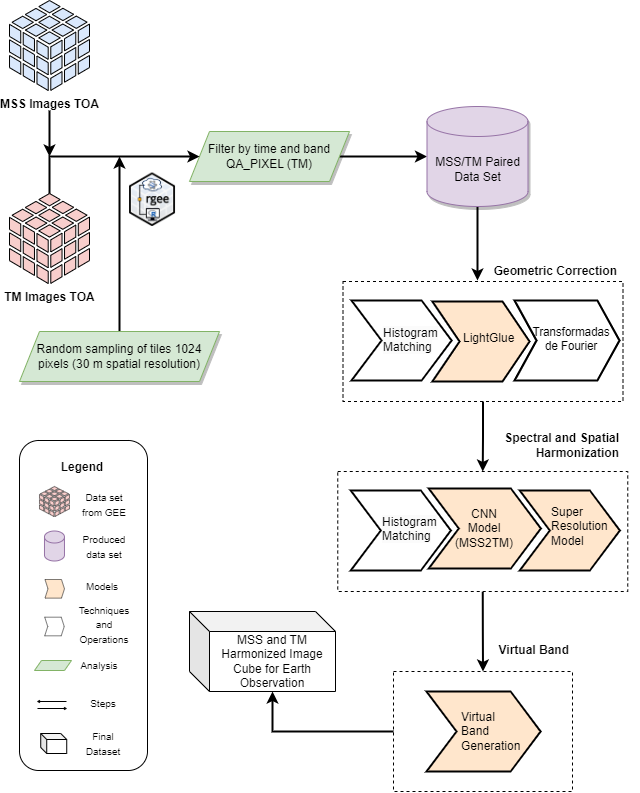
\includegraphics[width=0.95\linewidth]{2_CAPITULO0/IMG/modelo.png}
                \begin{justify}
                    \textit{Nota.} El esquema presenta una metodología de armonización de imágenes de sensores MSS y TM: comienza con imágenes TOA, sigue con correcciones geométricas y transformadas de Fourier via LightGlue, continúa con armonización espectral y espacial mediante modelos CNN y culmina con un cubo de imagen armonizado para la creación de bandas virtuales.
                \end{justify}                    
                \label{modelo}
            \end{figure}

    \section{Análisis estadístico}

        En la fase de preparación para la validación de los modelos desarrollados, se diseñó un enfoque de análisis estadístico detallado. Este diseño metodológico fue crucial para asegurar que, una vez aplicados, los modelos pudieran demostrar un ajuste adecuado a los datos de entrenamiento y una generalización efectiva a nuevos conjuntos de datos.
        
        Se decidió que el RMSE se calcularía para estimar la discrepancia entre las predicciones de los modelos y los valores observados, buscando valores bajos como indicativos de precisión. Además, se preveía el uso del coeficiente de correlación de Pearson para examinar la relación lineal entre las predicciones y los valores reales.
        
        En la fase de validación, se llevó a cabo una evaluación exhaustiva del modelo MSS2TM ESRGAN utilizando el conjunto de validación previamente definido. Este conjunto, compuesto por pares de imágenes MSS-TM, permitió una comparativa directa entre las imágenes superresueltas generadas por el modelo y las correspondientes imágenes de alta resolución (TM). Los pasos fundamentales en esta etapa incluyeron:

        \subparagraph{Evaluación de Métricas de Rendimiento}
            Se aplicaron diversas métricas para cuantificar la eficacia del modelo. Estas métricas incluyeron el Peak Signal-to-Noise Ratio (PSNR) y el Structural Similarity Index (SSIM), que proporcionan una medida cuantitativa del error y la calidad visual, respectivamente. Adicionalmente, se utilizó CLIPScore, una métrica más novedosa y alineada con la percepción visual humana, para evaluar la calidad perceptual de las imágenes superresueltas. Estas métricas son fundamentales para comprender cómo el modelo reproduce detalles y texturas específicas en las imágenes de superresolución.

        \paragraph{Comparación Visual}
            Además de la evaluación cuantitativa, se realizó una comparación visual detallada entre las imágenes generadas por el modelo y las imágenes TM de alta resolución. Esta comparación permitió identificar la efectividad del modelo en la recuperación de detalles finos y en la representación precisa de las características geoespaciales.